\section{结果}
\label{sec:results}

\subsection{已知真实值下的目标特异风险}
\label{sec:res-theory}

已知真实值的模拟呈现了模型预言的目标差异（图~\ref{fig:concept}）。报告概率固定且正确已知时，当期再生数的误差随病例量倒数下降；固定一组已实现时期的均值误差也下降，因为这些时期的真实波动属于目标本身。对于平稳过程均值，在抽取时期数固定时，误差保留实现均值的方差。模拟仅检查模型自身假设下的公式，并不证明住院统计量截距有相同来源。

采用平均报告率归一化、而当期完整度独立波动时，当期误差趋向报告项而非零。有限时期均值也继承除以独立时期数的报告分量。因此，没有环境底线不等于没有观察过程底线。模拟记录每项比较的蒙特卡洛标准误，按模拟不确定性评价数值差异，而不以任意百分比作为一致标准。附录~\ref{app:extensions} 的方差平衡和预算结果属于该指定模型，不是由住院数据识别的操作门槛。

\begin{figure}[tbp]
\centering
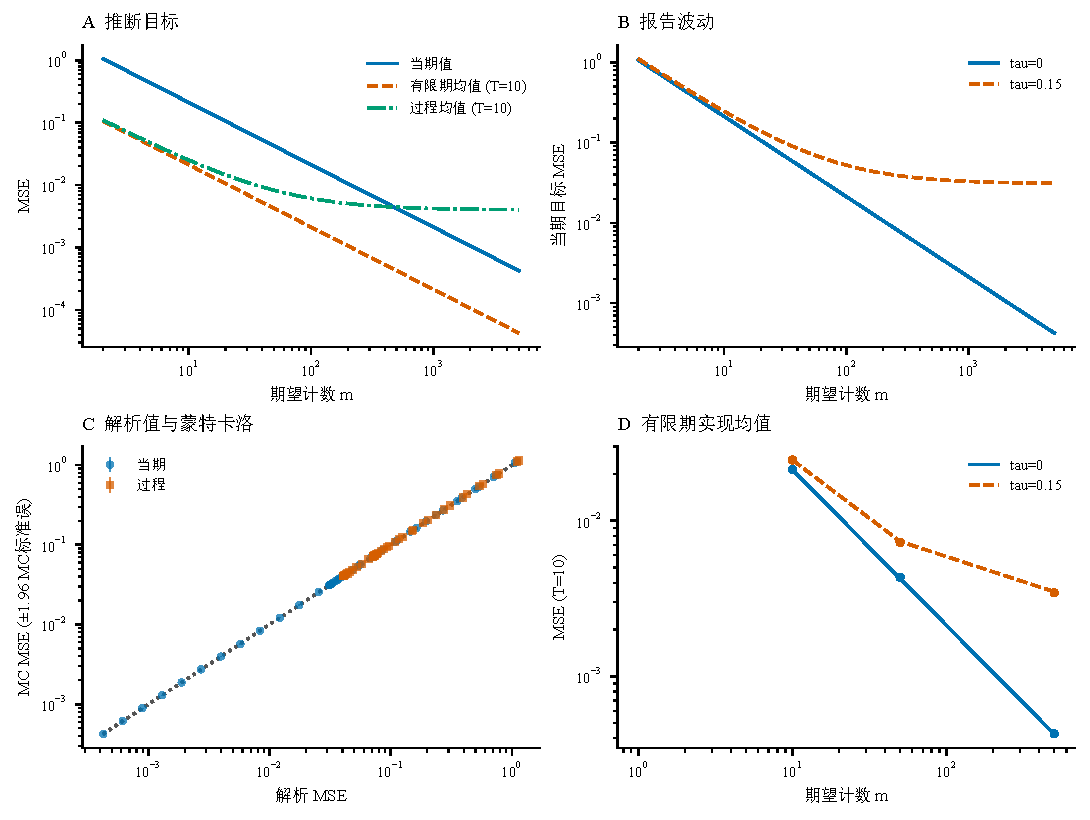
\includegraphics[width=\linewidth]{figures/fig_01_targets.pdf}
\caption{推断目标与报告假设。曲线为模型风险，图中点为已知真实值的蒙特卡洛检查。当期值和有限时期实现均值不同于平稳过程均值；不可测的时期报告波动也可给当期值留下非零风险。计数由声明的固定暴露模型生成，不代表在医院数据中识别出传播方差底线。}
\label{fig:concept}
\end{figure}

\subsection{观测损失曲线与留出比较}
\label{sec:res-empirical}

重建后的主 $R_A$ 样本包含 \Nra{} 个州周。仿射工作模型得到 $a=\RAaPoint{}$（95\% 区间 \RAaInterval{}）、$b=\RAbPoint{}$（\RAbInterval{}）及表观比值 $b/a=\RAratioPoint{}$（\RAratioInterval{}）。$G$ 的对应比值为 \GratioPoint{}（\GratioInterval{}；表~\ref{tab:pooled}）。这些估计描述指定仿射形式下表观统计量的相对离散程度；正条件截距不确定观测病例范围之外的曲线形式。

两个工作模型都描述了支持范围内损失的大体变化，但留出预测排名并不一致（图~\ref{fig:model-comparison}；表~\ref{tab:cv}）。$R_A$ 的幂律减仿射平均评分，在逐州留出时为 \RAstateCVPoint{}，逐季留出时为 \RAseasonCVPoint{}：前者为负，有利于幂律；后者为正，有利于仿射。$G$ 的两项摘要均有利于幂律，分别为 \GstateCVPoint{} 和 \GseasonCVPoint{}。比较全程使用训练折中心。各折结果单独保留，因为较小的汇总差异掩盖了留出情景之间的变化，仅四个季节也只能有限评价新流行机制中的泛化。

正拟合截距与这种混合预测排序都没有独立确立不变的传播方差平台。因此，$b/a$ 仅作为仿射描述量。表~\ref{tab:pooled} 的 3.2 天变换敏感性区分了表观统计量定义改变与模拟器真实间隔改变，不能据此判定住院数据由哪个间隔生成。补充设计实验评价声明的合成曲线之可区分性；部分设定下较高功效不能替代实证检验，零假设留出拒绝率与功效一并报告。

\begin{figure}[tbp]
\centering
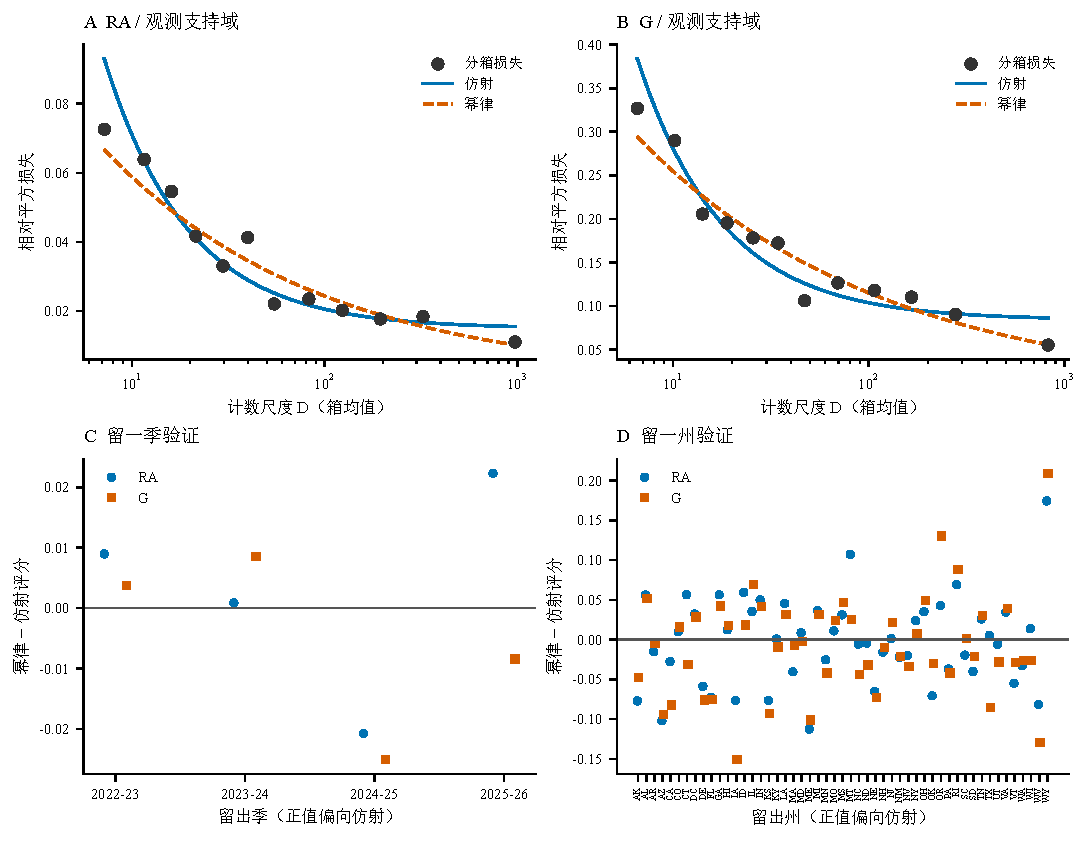
\includegraphics[width=\linewidth]{figures/fig_02_models.pdf}
\caption{经验支持范围与留出曲线比较。分箱均值描述观测病例量范围内的相对损失，不作为独立观测或未聚类显著性检验。仿射与幂律均为拟合工作模型。测试评分使用训练折内估计的中心和模型参数，幂律减仿射评分为正时有利于仿射，为负时有利于幂律。各折不是独立重复。}
\label{fig:model-comparison}
\end{figure}

\subsection{对受控随机移除病例的响应}
\label{sec:res-thinning}

对 $R_A$ 样本（n=\Nra{} 个州周），全保留率水平的稀释速率为 \ThinAllPoint{}（95\% 区间 \ThinAllInterval{}），近似弹性参照为 \ThinBPPoint{}，与参照的配对比值为 \ThinRatioPoint{}（\ThinRatioInterval{}）。剔除最极端保留率后得到 \ThinNoqPoint{}（\ThinNoqInterval{}；图~\ref{fig:thinning}、表~\ref{tab:thinning}）。二者值得并列考察，因为 $q=0.1$ 对过原点回归预测变量平方和的贡献约为 76\%。这来自所选逆保留率设计，本身不证明该点存在偏差。

原始 $C_t\ge50$ 子样本的速率为 \ThinHighPoint{}（\ThinHighInterval{}），同时要求当前和下一周计数均不低于 50 时为 \ThinBothPoint{}（\ThinBothInterval{}）。后一限制处理了前一限制的不足：较大的当前计数不保证稀释后的分子也足够大。所有子样本均由原始计数确定，不在稀释后重新筛选；每个子样本使用重新计算的参照系数，不借用全样本值。

图~\ref{fig:thinning} 同时报告截距差及联合不确定性，包括低保留率下的偏离。区间包含零不表示截距严格不变。即使施加的计数移除机制已知，非线性变换、连续性修正、重新中心化与回归仍可影响拟合响应。补充输出中的已知泊松计数例检查完整流程，不声称代表现实中的全部报告机制。

计算实际使用 \ThinBootstrap{} 次外层样本、\ThinPointReps{} 次点实现，每个外层水平使用 \ThinInnerReps{} 次内层实现。表~\ref{tab:thinning} 报告预定蒙特卡洛检查及拟合失败，由于点估计平均的实现次数多于每个自助抽样，区间同时包含抽样变异与有限内层模拟波动；表~
ef{tab:thinning} 报告两部分误差、预定蒙特卡洛检查与拟合失败。实验刻画这些已记录病例对进一步随机移除的响应，不分离原截距中的传播、住院实践、延迟观察和报告变异；$b(1)$ 与 $c_{\rm thin}$ 的差额也不唯一量化后代过度离散。

\begin{figure}[tbp]
\centering
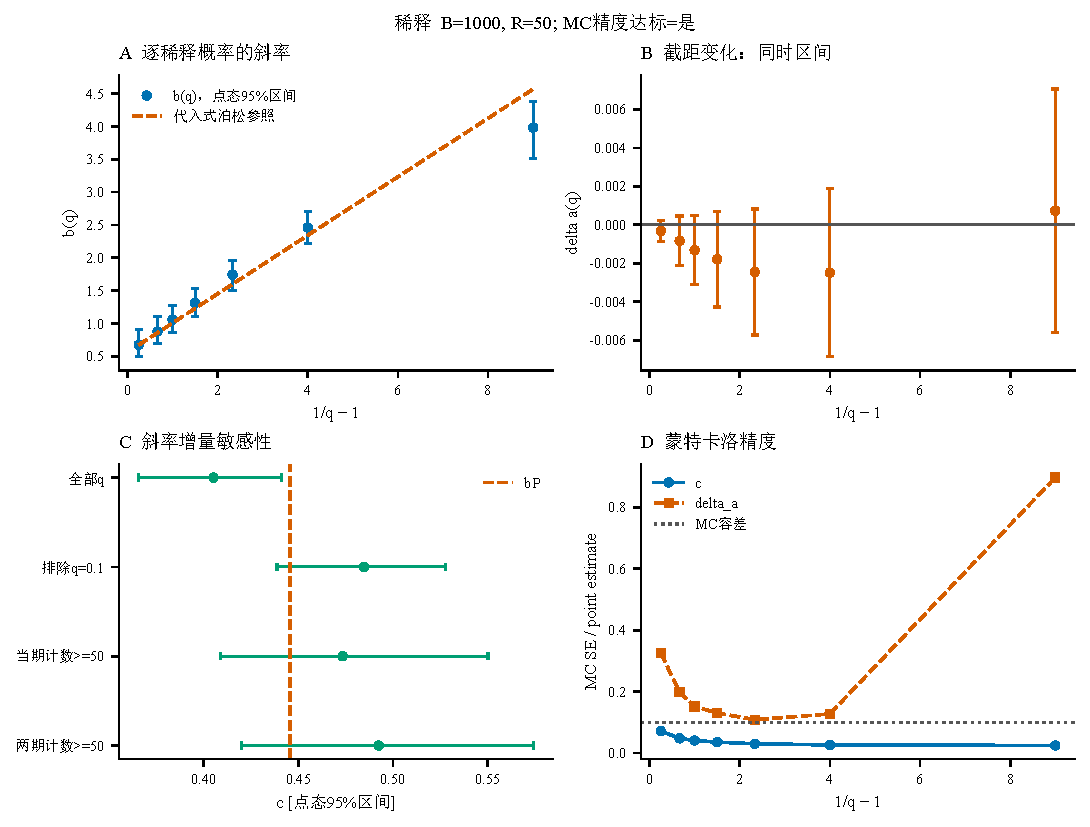
\includegraphics[width=\linewidth]{figures/fig_03_thinning.pdf}
\caption{固定样本上的受控稀释。重新计算统计量和中心后，在原始病例尺度上拟合系数。截距差区间带考虑不同保留率间的联合自助变异。敏感性包括全部水平、剔除 $q=0.1$，以及限制原始当前和下一周计数。泊松弹性系数是近似参照，不是所有非线性拟合系数的精确预测。实际内外层重复次数见表~\ref{tab:thinning}。}
\label{fig:thinning}
\end{figure}

\subsection{州异质性与损失参照选择}
\label{sec:res-fe}

对同一样本（$R_A$，n=\Nra{}），包含州截距和共同州内斜率时，$b_{\rm w}=\FEbPoint{}$（\FEbInterval{}），州截距均值为 \FEaPoint{}（\FEaInterval{}）。均值口径的比值为 \FEratioPoint{}（\FEratioInterval{}）；采用实际加权 $D_t$ 得到 \FEDratioPoint{}（\FEDratioInterval{}；图~\ref{fig:heterogeneity}、表~\ref{tab:fe}）。后一规格是独立拟合，不再是单周计数分析的别名。

独立重抽样日历周时，合并对州内的配对比值为 \FEpairedPoint{}（\FEpairedInterval{}）。两周、三周块区间分别为 \FEpairedBlockTwoInterval{} 和 \FEpairedBlockThreeInterval{}。普通区间下界略高于 1，时间块区间则包含 1。因此差异依赖于如何表示时间相关，不能转换为空间汇总的因果贡献比例。主州模型在 \FEBootstrap{} 次自助样本中有 \FEvalid{} 次有效拟合，有限有效重复区间的条件性及诊断失败均已标注。州与周双向点诊断未达到数值收敛标准，不报告斜率或置信区间。

改变损失参照同样会改变截距（表~\ref{tab:centering}）。保持共同全局归一化分母，用全国周中心替代合并中心后，$R_A$ 截距减少 \RAweekReductionPoint{}\%（\RAweekReductionInterval{}\%），$G$ 减少 \GweekReductionPoint{}\%（\GweekReductionInterval{}\%）。该降幅仅针对固定归一化分母；若同时改变归一化，将定义另一个不可直接比较的量。按季中心化与共同线性去趋势并不产生相同变化。不同参照移除不同的观测轨迹成分，其中包含真实共同信号。排除自身州的变体进一步记录一个观测参与自身周参照的影响。这些比较刻画定义敏感性，不构成独立传播与报告方差的已识别分解。

\begin{figure}[tbp]
\centering
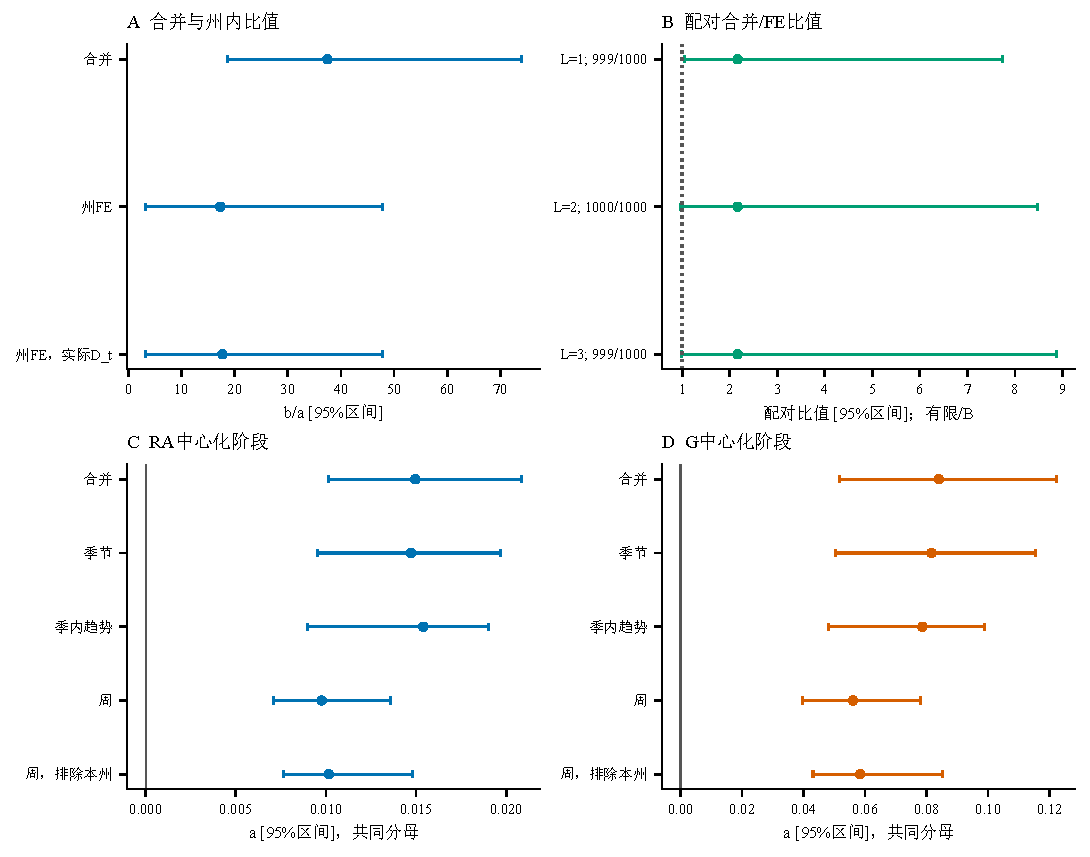
\includegraphics[width=\linewidth]{figures/fig_04_heterogeneity.pdf}
\caption{空间规格与参照敏感性。合并和州截距估计使用相同的全局损失定义；$D_t$ 敏感性使用加权滞后计数。参照调整保持全局归一化不变，仅改变中心或共同趋势。时间块配对区间展示对时间依赖处理的敏感性。未定义或未收敛结果不绘制成有效估计；不同参照对应不同经验目标。}
\label{fig:heterogeneity}
\end{figure}

\subsection{条件校准的限制}
\label{sec:res-sim}

补充校准对两种表观统计量使用修正后的观察机制，报告全部声明情景（表~\ref{tab:calibration}）。其中区分来源匹配的 3.2 天、标准差 2.1 天间隔，固定变异系数敏感性，以及历史 3.6 天代理。条件区间合并配对经验与模拟器不确定性，不对假造的间隔假设分布取平均。

模拟器可以重现截距，却不能同时重现斜率或有效样本量。因此响应检查保留这些差异，不通过抬高初始零计数或选择有利情景消除它们。初始条件和无输入感染的假设可使初始为零的州之后仍无感染，这不同于持续存在输入的现实监测。全国与州持续性、计数过度离散、报告波动在模拟器中也是不同机制；多个摘要相容并不能唯一识别其中一个。本文不据校准值断言有固定比例的真实州周超过生物学或经济门槛。
